\documentclass[tikz, border=6pt]{standalone}
\IfFileExists{lmodern.sty}{\usepackage[T1]{fontenc}\usepackage{lmodern}}{}
\usepackage{amsmath,amssymb,bm}
\usepackage[scaled=0.95]{helvet}
\usetikzlibrary{arrows.meta}
\definecolor{Blue}{HTML}{3A76D8}
\definecolor{Orange}{HTML}{EE8133}
\definecolor{Red}{HTML}{DF4B4B}
\definecolor{Ink}{HTML}{1F2937}
\begin{document}
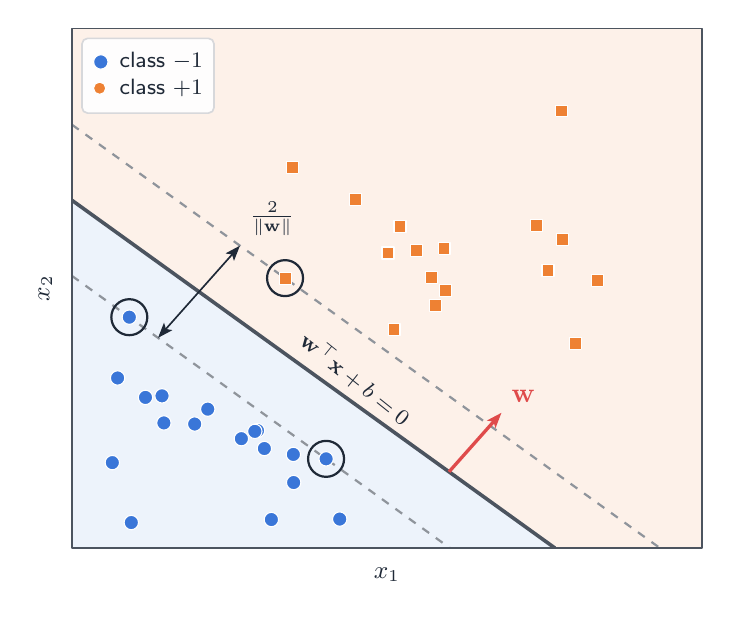
\begin{tikzpicture}[color=Ink, execute at begin picture={\sffamily}, line width=0.6pt, >={Stealth[length=5.5pt, width=4pt, inset=1.2pt]}, line join=round]
  % axes ax1
  \begin{scope}
    \clip (0,0) rectangle (8,6.6);
    \begin{scope}
      \clip (0,0) rectangle (8,6.6);
      \fill[Blue!9, even odd rule] (0,0) -- (0,4.407) -- (0.04,4.407) -- (0.161,4.286) -- (0.201,4.286) --
          (0.322,4.165) -- (0.362,4.165) -- (0.442,4.085) -- (0.482,4.085) -- (0.603,3.964) --
          (0.643,3.964) -- (0.724,3.884) -- (0.764,3.884) -- (0.884,3.763) -- (0.925,3.763) --
          (1.005,3.682) -- (1.045,3.682) -- (1.166,3.562) -- (1.206,3.562) -- (1.327,3.441) --
          (1.367,3.441) -- (1.447,3.36) -- (1.487,3.36) -- (1.608,3.24) -- (1.648,3.24) -- (1.729,3.159)
          -- (1.769,3.159) -- (1.889,3.038) -- (1.93,3.038) -- (2.01,2.958) -- (2.05,2.958) --
          (2.171,2.837) -- (2.211,2.837) -- (2.291,2.757) -- (2.332,2.757) -- (2.452,2.636) --
          (2.492,2.636) -- (2.613,2.515) -- (2.653,2.515) -- (2.734,2.435) -- (2.774,2.435) --
          (2.894,2.314) -- (2.935,2.314) -- (3.015,2.234) -- (3.055,2.234) -- (3.176,2.113) --
          (3.216,2.113) -- (3.296,2.032) -- (3.337,2.032) -- (3.457,1.912) -- (3.497,1.912) --
          (3.618,1.791) -- (3.658,1.791) -- (3.739,1.71) -- (3.779,1.71) -- (3.899,1.59) -- (3.94,1.59) --
          (4.02,1.509) -- (4.06,1.509) -- (4.181,1.388) -- (4.221,1.388) -- (4.302,1.308) -- (4.342,1.308)
          -- (4.462,1.187) -- (4.503,1.187) -- (4.583,1.107) -- (4.623,1.107) -- (4.744,0.986) --
          (4.784,0.986) -- (4.905,0.865) -- (4.945,0.865) -- (5.025,0.785) -- (5.065,0.785) --
          (5.186,0.664) -- (5.226,0.664) -- (5.307,0.584) -- (5.347,0.584) -- (5.467,0.463) --
          (5.508,0.463) -- (5.588,0.382) -- (5.628,0.382) -- (5.749,0.262) -- (5.789,0.262) --
          (5.869,0.181) -- (5.91,0.181) -- (6.03,0.06) -- (6.07,0.06) -- (6.131,0) -- cycle;
      \fill[Orange!11, even odd rule] (6.151,0) -- (6.131,0) -- (6.07,0.06) -- (6.03,0.06) -- (5.91,0.181)
          -- (5.869,0.181) -- (5.789,0.262) -- (5.749,0.262) -- (5.628,0.382) -- (5.588,0.382) --
          (5.508,0.463) -- (5.467,0.463) -- (5.347,0.584) -- (5.307,0.584) -- (5.226,0.664) --
          (5.186,0.664) -- (5.065,0.785) -- (5.025,0.785) -- (4.945,0.865) -- (4.905,0.865) --
          (4.784,0.986) -- (4.744,0.986) -- (4.623,1.107) -- (4.583,1.107) -- (4.503,1.187) --
          (4.462,1.187) -- (4.342,1.308) -- (4.302,1.308) -- (4.221,1.388) -- (4.181,1.388) --
          (4.06,1.509) -- (4.02,1.509) -- (3.94,1.59) -- (3.899,1.59) -- (3.779,1.71) -- (3.739,1.71) --
          (3.658,1.791) -- (3.618,1.791) -- (3.497,1.912) -- (3.457,1.912) -- (3.337,2.032) --
          (3.296,2.032) -- (3.216,2.113) -- (3.176,2.113) -- (3.055,2.234) -- (3.015,2.234) --
          (2.935,2.314) -- (2.894,2.314) -- (2.774,2.435) -- (2.734,2.435) -- (2.653,2.515) --
          (2.613,2.515) -- (2.492,2.636) -- (2.452,2.636) -- (2.332,2.757) -- (2.291,2.757) --
          (2.211,2.837) -- (2.171,2.837) -- (2.05,2.958) -- (2.01,2.958) -- (1.93,3.038) -- (1.889,3.038)
          -- (1.769,3.159) -- (1.729,3.159) -- (1.648,3.24) -- (1.608,3.24) -- (1.487,3.36) --
          (1.447,3.36) -- (1.367,3.441) -- (1.327,3.441) -- (1.206,3.562) -- (1.166,3.562) --
          (1.045,3.682) -- (1.005,3.682) -- (0.925,3.763) -- (0.884,3.763) -- (0.764,3.884) --
          (0.724,3.884) -- (0.643,3.964) -- (0.603,3.964) -- (0.482,4.085) -- (0.442,4.085) --
          (0.362,4.165) -- (0.322,4.165) -- (0.201,4.286) -- (0.161,4.286) -- (0.04,4.407) -- (0,4.407) --
          (0,6.6) -- (8,6.6) -- (8,0) -- cycle;
    \end{scope}
    \draw[color=Ink!80, line width=1.3pt] (0,4.416) -- (6.133,0);
    \draw[dashed, color=Ink!50, line width=0.8pt] (0,5.376) -- (7.467,0);
    \draw[dashed, color=Ink!50, line width=0.8pt] (0,3.456) -- (4.8,0);
    \filldraw[fill=Blue, draw=white, line width=0.4pt] (2.356,1.492) circle[radius=2.6pt];
    \filldraw[fill=Blue, draw=white, line width=0.4pt] (2.151,1.389) circle[radius=2.6pt];
    \filldraw[fill=Blue, draw=white, line width=0.4pt] (1.143,1.933) circle[radius=2.6pt];
    \filldraw[fill=Blue, draw=white, line width=0.4pt] (0.512,1.085) circle[radius=2.6pt];
    \filldraw[fill=Blue, draw=white, line width=0.4pt] (0.579,2.16) circle[radius=2.6pt];
    \filldraw[fill=Blue, draw=white, line width=0.4pt] (0.933,1.913) circle[radius=2.6pt];
    \filldraw[fill=Blue, draw=white, line width=0.4pt] (1.558,1.575) circle[radius=2.6pt];
    \filldraw[fill=Blue, draw=white, line width=0.4pt] (2.811,1.189) circle[radius=2.6pt];
    \filldraw[fill=Blue, draw=white, line width=0.4pt] (1.167,1.589) circle[radius=2.6pt];
    \filldraw[fill=Blue, draw=white, line width=0.4pt] (3.4,0.368) circle[radius=2.6pt];
    \filldraw[fill=Blue, draw=white, line width=0.4pt] (2.443,1.264) circle[radius=2.6pt];
    \filldraw[fill=Blue, draw=white, line width=0.4pt] (0.753,0.324) circle[radius=2.6pt];
    \filldraw[fill=Blue, draw=white, line width=0.4pt] (2.322,1.482) circle[radius=2.6pt];
    \filldraw[fill=Blue, draw=white, line width=0.4pt] (1.724,1.764) circle[radius=2.6pt];
    \filldraw[fill=Blue, draw=white, line width=0.4pt] (2.532,0.362) circle[radius=2.6pt];
    \filldraw[fill=Blue, draw=white, line width=0.4pt] (2.815,0.832) circle[radius=2.6pt];
    \filldraw[fill=Orange, draw=white, line width=0.4pt] (6.14,5.475) rectangle (6.292,5.626);
    \filldraw[fill=Orange, draw=white, line width=0.4pt] (4.65,3.725) rectangle (4.801,3.877);
    \filldraw[fill=Orange, draw=white, line width=0.4pt] (4.543,3.009) rectangle (4.695,3.161);
    \filldraw[fill=Orange, draw=white, line width=0.4pt] (5.969,3.45) rectangle (6.121,3.602);
    \filldraw[fill=Orange, draw=white, line width=0.4pt] (4.666,3.195) rectangle (4.818,3.347);
    \filldraw[fill=Orange, draw=white, line width=0.4pt] (4.015,2.701) rectangle (4.166,2.853);
    \filldraw[fill=Orange, draw=white, line width=0.4pt] (6.149,3.847) rectangle (6.301,3.999);
    \filldraw[fill=Orange, draw=white, line width=0.4pt] (5.819,4.018) rectangle (5.971,4.17);
    \filldraw[fill=Orange, draw=white, line width=0.4pt] (3.937,3.671) rectangle (4.089,3.823);
    \filldraw[fill=Orange, draw=white, line width=0.4pt] (4.089,4.012) rectangle (4.241,4.164);
    \filldraw[fill=Orange, draw=white, line width=0.4pt] (4.299,3.698) rectangle (4.451,3.85);
    \filldraw[fill=Orange, draw=white, line width=0.4pt] (6.599,3.319) rectangle (6.751,3.471);
    \filldraw[fill=Orange, draw=white, line width=0.4pt] (3.529,4.348) rectangle (3.681,4.5);
    \filldraw[fill=Orange, draw=white, line width=0.4pt] (6.319,2.521) rectangle (6.471,2.673);
    \filldraw[fill=Orange, draw=white, line width=0.4pt] (4.488,3.359) rectangle (4.64,3.511);
    \filldraw[fill=Orange, draw=white, line width=0.4pt] (2.728,4.754) rectangle (2.88,4.906);
    \filldraw[fill=Blue, draw=white, line width=0.4pt] (3.227,1.133) circle[radius=2.6pt];
    \filldraw[fill=Blue, draw=white, line width=0.4pt] (0.728,2.932) circle[radius=2.6pt];
    \filldraw[fill=Orange, draw=white, line width=0.4pt] (2.63,3.352) rectangle (2.782,3.504);
  \end{scope}
  \draw[Ink!80, line width=0.5pt] (0,0) rectangle (8,6.6);
  \node[rotate=-38.6598, anchor=south, font=\footnotesize] at (3.435,1.943) {$\mathbf{w}^\top\mathbf{x} + b = 0$};
  \node[anchor=north, font=\small, align=center, inner sep=4pt] at (4,-0.1) {$x_1$};
  \node[anchor=south, rotate=90, font=\small, align=center, inner sep=4pt] at (-0.1,3.3) {$x_2$};
  \node[anchor=north west, font=\footnotesize, inner sep=4pt, align=left, fill=white, draw=Ink!18, rounded corners=2pt, fill opacity=0.92, text opacity=1] at (0.12,6.48) {%
    \begin{tabular}{@{}l@{\hspace{4pt}}l@{}}
      \tikz[baseline=-0.6ex]{\filldraw[fill=Blue, draw=white, line width=0.4pt] (0.3,0) circle[radius=2.6pt];} & class $-1$ \\
      \tikz[baseline=-0.6ex]{\filldraw[fill=Orange, draw=white, line width=0.4pt] (0.224,-0.076) rectangle (0.376,0.076);} & class $+1$ \\
    \end{tabular}%
  };
  \draw[draw=Ink, line width=0.8pt] (3.2267,1.1328) circle[radius=6.5pt];
  \draw[draw=Ink, line width=0.8pt] (0.7279,2.9319) circle[radius=6.5pt];
  \draw[draw=Ink, line width=0.8pt] (2.7056,3.428) circle[radius=6.5pt];
  \draw[<->, color=Ink] (1.0923,2.6695) -- (2.133,3.8403);
  \node[anchor=south west, font=\small] at (2.133,3.8403) {$\frac{2}{\|\mathbf{w}\|}$};
  \draw[->, color=Red, line width=1.2pt] (4.7882,0.9685) -- (5.4545,1.7182);
  \node[anchor=south west, text=Red] at (5.4545,1.7182) {$\mathbf{w}$};
\end{tikzpicture}
\end{document}
